\chapter{Results}

%----------------------------------------------------------------------------------------------------------------------

\noindent
The results that we gathered were based on a number of sample environments which a simulated robot then traversed. A large number of our tests were conducted using a mock office floor plan of $12m^{2}$ containing $0.3m^{2}$ cells seen in Figure \ref{path_comparison}. The start and end points were placed on opposite sides of the map forcing the mobile robot to traverse the longest possible paths. For each sample environment we looked at every possible path to the selected goal by considering all of the free cells. From this we collected a large amount of data which was then analysed to determine which planner produced the shortest paths on average.

\begin{figure}[htbp]

\center 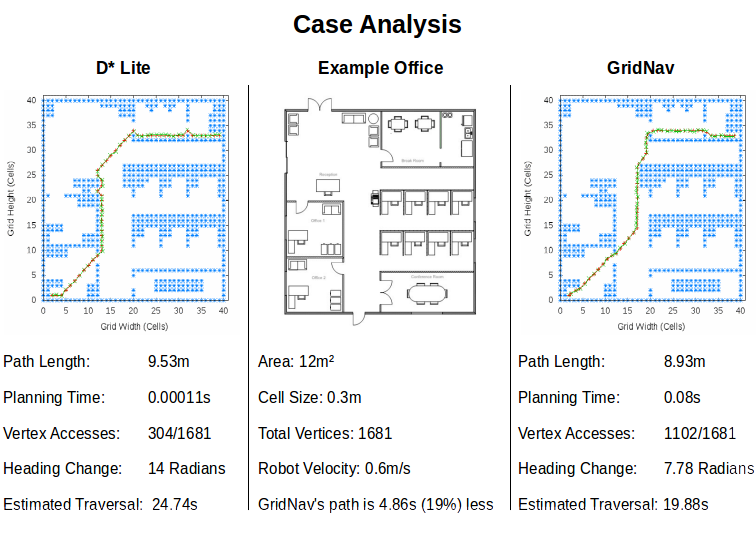
\includegraphics[width=250pt]{illustrations/floor_plan}\\
\caption{A case analysis based on the sample office environment used during testing.} 
\label{path_comparison}

\end{figure}

\section{Statistical Analysis}
\noindent
During the analysis phase we looked at a total of 4,600 test cases, 1,200 per planner. We used a combination of each planner's average performance and their worst case scenario to established a ranking. For each planner we produced a standard dataset containing estimated traversal and computation times, these datasets were then imported into RStudio and analysed using R. We found all the datasets to be evenly distributed as their means and median values differed by little, also longer path lengths required more computations, although this relationship is not linear. Below is part of our RScript: \\

\begin{lstlisting}
##### Analysis of Grid Nav #####

# Get worst case scenario
val = max(gridnav$traverse)
index = which(gridnav$traverse == val)
gridnav[index, ]

gridnav_accesses_mean = mean(gridnav$accesses)
median(gridnav$accesses)

gridnav_traverse_mean = mean(gridnav$traverse)
median(gridnav$traverse)

gridnav_total_mean = gridnav_accesses_mean + gridnav_traverse_mean

[output omitted]

# Calculate how much more efficient planners are than D* Lite
100 - (gridnav_total_mean / (d_star_lite_total_mean / 100))
100 - (theta_star_total_mean / (d_star_lite_total_mean / 100))
100 - (field_d_star_total_mean / (d_star_lite_total_mean / 100))
\end{lstlisting}

\noindent
Based on our analysis we came up with the following ranking for the planners in terms of efficiency:

\begin{enumerate}
\item Theta*
\item GridNav
\item Field D*
\item D* Lite
\end{enumerate}

\noindent
The top three planners outperformed D* Lite by at least 10\% and differed from each other by around 1\%. Theta*'s \textit{ray casting} approach produced shorter paths than either GridNav or Field D* however they were also angular in nature (see Figure \ref{floor_plan}). Such direct paths require a mobile robot to perform extremely sharp changes in direction which can be impractical when operating in confined environments. While Theta* may produce the shortest possible paths GridNav's smoother paths are easier to execute.

\begin{figure}[htbp]

\center 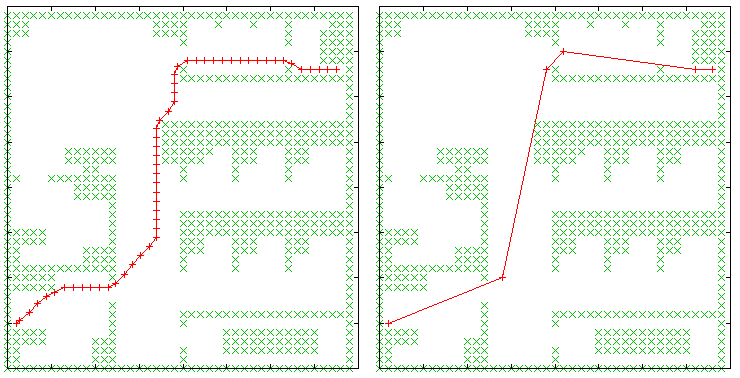
\includegraphics[width=250pt]{illustrations/comparison}\\
\caption{Output from GridNav (left) and Theta* (right), Theta*'s path is shorter to traverse but also more angular which may not suit all forms of locomotion.} 
\label{floor_plan}

\end{figure}

\noindent
GridNav uses a simple yet effective heading calculator based on \textit{gradient descent} which works much like the way a stream finds its way down a mountain \cite{GRIDNAV95}. It has the advantage over Field D* as gradient descent has proved easier to implement than a linear interpolation heading calculator. It also does not require significant changes to the underlying graph representation as is required with Field D*.

\newpage

\section{Significance of Findings}
We found that Theta*, GridNav, and Field D*, all planners that are not restricted to a small set of headings, could be up to 10\% more efficient than D* Lite. Meaning that travel time, energy consumption, and mechanical wear can be reduced significantly by adopting any planner that is not limited to headings of $\dfrac{\pi}{4}$. This can be very significant if we consider journeys that require a robot to travel long distances. For some of our test cases D* Lite produced paths that were several metres longer than its competitors. This meant the robot had to travel an extra distance simply because of D* Lite's limitations regarding heading changes.  \\

\noindent
One argument against these natural path planners is that computationally they are less efficient. They require complex representations of the environment and more vertex accesses, in some cases in excess of 96\% more time is spent computing a path \cite{FIELD}. For any of our tests we found that less than 1\% of a journey's time was spent planning the path, meaning the other 99\% was used on travelling. A planners computation time does not represent a significant proportion of the overall process. The difference in computation time may be measured in milliseconds but this is easily cancelled out in cases where the traversal time differs by tens of seconds. Scaling up the environment has no impact on the performance as the faster planner still suffers from suboptimal paths that are difficult to traverse in practice.